
\labday{Lundi, 11 avril 2016}
\label{day:11-04-2016}

{\Large \textbf{Vocabulaire}}

L'objectif de ces expériences est d'arriver à associer entre-elles des données
provenant de distributions très similaires.

On dispose d'un jeu de donnée \textbf{Source} qui contient les données 
\textbf{Originales}, \textbf{Non biaisées} ou encore proviennent de
la \textbf{Réalité}.

Ce jeu de donnée est opposé aux données \textbf{Cible} qui contiennent des
données \textbf{Transformées}, \textbf{biaisées} ou encore proviennent de
\textbf{Simulations}.

On cherche ici à construire un \textbf{correcteur} qui va rapprocher/projeter
les données \emph{Cibles} sur les données \emph{Sources} correspondantes.

On note $\mathcal{X_S}$ les données sources, $\mathcal{X_T}$ les données 
cibles (Target) et $\mathcal{Y}$ les labels (s'il y en a).

On note $\phi$ la fonction inconnue qui a transformé/biaisé les données \emph{Cible}.
\begin{align*}
\phi : \mathcal{X_S}  &\to \mathcal{X_T} \\
                  x &\mapsto x^\prime
\end{align*}

Et $\psi$ la fonction que notre modèle va apprendre. On espère obtenir
$\phi \circ \psi = identity$.



\experiment{Apprendre l'alignement : résumé des idées et discussions}

Je résume ici une discussion sur les problèmes et solutions sur l'algorithme
visant à apprendre l'alignement pendant l'entraînement du correcteur.

\subexperiment{Brute Force}

Commençons par rappeler l'algo \emph{brute force} que l'on va par la suite
tenter d'améliorer.

L'idée précédente était d'utiliser les classes ou les sous-classes connues
afin de tenter d'aligner les données. 

\begin{algorithm}[tb]
   \caption{Alignement aléatoire}
   \label{alg:align_random}
\begin{algorithmic}
    \State {\bfseries Entrée:} données cible $\mathcal{X_T}$, données cibles $\mathcal{X_S}$, classes $\mathcal{Y}$
    \State \textcolor{gray}{Initialisation :}
    \State $c \gets $ nombre de classe dans $\mathcal{Y}$
    \State $n \gets $ nombre d'exemple dans $\mathcal{X_T}$
    \State $NN \gets$ réseau de neurone initialisé
    \While{Convergence ou temps écoulé}
        \State \textcolor{gray}{Réorganiser aléatoirement l'alignement en respectant les classes :}
        \State $idx \gets \text{array}(n)$
        \For{$i=0$ {\bfseries to} $c$}
            \State $idx_i \gets \text{where}(\mathcal{Y}=i)$
            \State $idx_i^\prime \gets \text{shuffle}(idx_i)$
            \State $idx[idx_i]\gets idx_i^\prime$
        \EndFor
        \State $\mathcal{X_T} \gets \mathcal{X_T}[idx]$
        \State \textcolor{gray}{Entraîner le réseaux pour 1 époque :}
        \State $NN.\text{train}(\mathcal{X}, \mathcal{X_S})$
    \EndWhile
    \State {\bfseries Rendre} le réseaux
\end{algorithmic}
\end{algorithm}

Cela permet en effet de ramener des distributions `en paquet' correctement 
(figure \ref{fig:cloud_rotated_classwise})

\begin{figure}[H] % images
\centering
\subfigure[Corrected data]
    {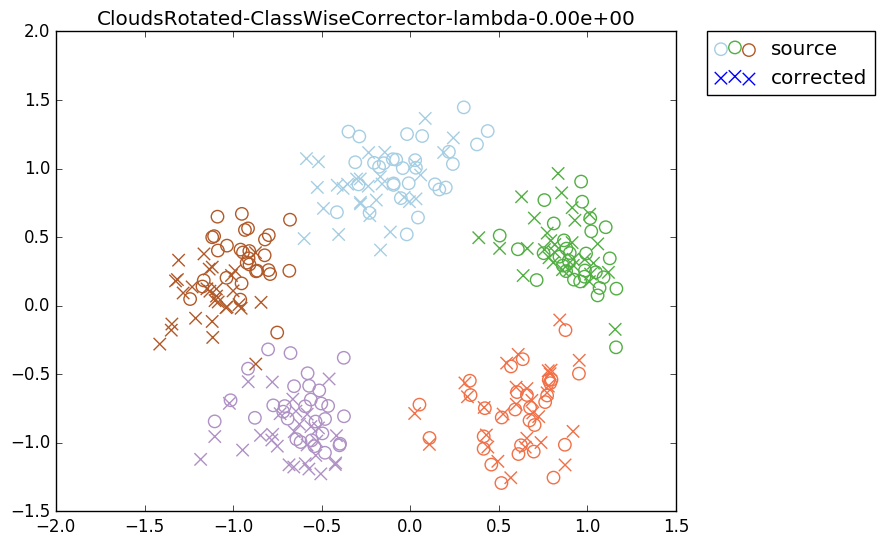
\includegraphics[width=0.45\linewidth]{fig/11-04-2016/CloudsRotated-ClassWiseCorrector-lambda-0.00e+00-corrected_data.png}}
\hfill
\subfigure[Target Data (uncorrected)]
    {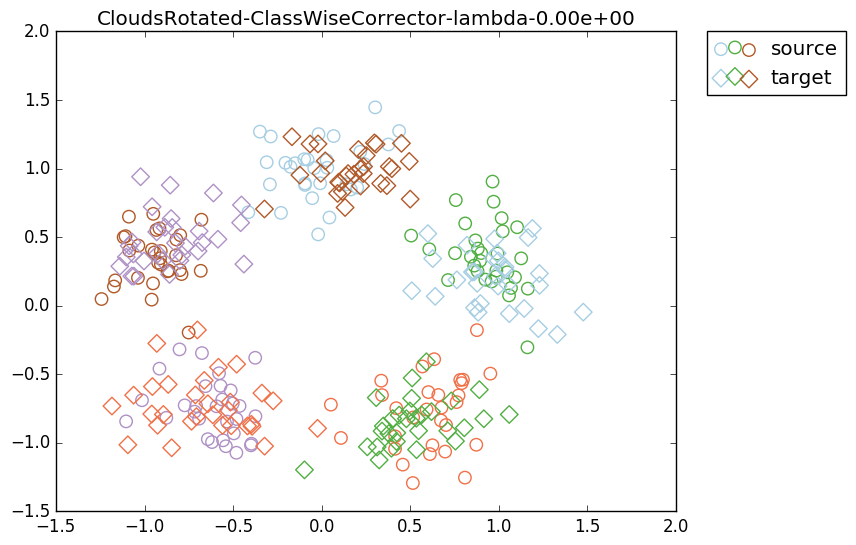
\includegraphics[width=0.45\linewidth]{fig/11-04-2016/CloudsRotated-ClassWiseCorrector-lambda-0.00e+00-target_data.png}}
\caption{Clouds - Rotated }
\label{fig:cloud_rotated_classwise}
\end{figure}


Cependant comme vu précédemment (section \ref{exp:moon_0}) dans le cas de
distribution qui ne sont pas de simples nuages de point `gentils' cette approche 
peut mener à écraser les données corrigées sur le centre des distributions.
L'idée est donc d'apprendre l'alignement afin de faire mieux que rapprocher les
données du centre des distributions Source.

Plutôt que d'aligner aléatoirement les données entre chaque époque on va chercher
les éléments de la \emph{Source} qui correspondent le plus ou sont plus proche de 
ceux provenant de la \emph{Cible}. Il nous faut donc une distance : 
$$ \Delta : x, x^\prime \mapsto distance(x, x^\prime)$$

La première idée d'algorithme serait de d'aligner les données \emph{Cibles} avec leur
plus proche voisin dans les données \emph{Sources}. Cependant une solution triviale
alignant tous les exemples de la \emph{Cible} sur un seul et même exemple de la 
\emph{Source} est à éviter.

Pour éviter cette solution il faut forcer les exemples de la \emph{Cible} à s'aligner 
sur des exemples différents de la \emph{Source}.
On considère donc les $k$ plus proches voisins de chaque élément $x_T$ de la \emph{Cible}
Puis on l'aligne sur le plus proche voisin qui a été le moins choisis jusqu'à présent.


\begin{algorithm}[tb]
   \caption{Alignement KNN (K Nearest Neighbors)}
   \label{alg:align_KNN}
\begin{algorithmic}
    \State {\bfseries Entrée:} données cible $\mathcal{X_T}$, données cibles $\mathcal{X_S}$, classes $\mathcal{Y}$
    
    \Function{k-closest}{$x, X_S$} 
    \State $n \gets $ nombre d'exemple dans $\mathcal{X_S}$
    \State $closest \gets \text{array}(n)$
    \For{$i=0$ {\bfseries to} $n$}
        \State $closest[i] \gets \Delta(x, X_S[i])$
    \EndFor           
    \EndFunction

    \State \textcolor{gray}{Initialisation :}
    \State $c \gets $ nombre de classe dans $\mathcal{Y}$
    \State $n \gets $ nombre d'exemple dans $\mathcal{X_T}$
    \State $NN \gets$ réseau de neurone initialisé
    \While{Convergence ou temps écoulé}
        \State \textcolor{gray}{Réorganiser aléatoirement l'alignement en respectant les classes :}
        \State $idx \gets \text{array}(n)$
        \For{$i=0$ {\bfseries to} $c$}
            \State $idx_i \gets \text{where}(\mathcal{Y}=i)$
            \For{$j=0$ {\bfseries to} $n$}
                \State $closest \gets \textsc{k-closest}(\mathcal{X_T}[j], \mathcal{X_T})$
            \EndFor
            \State $idx[idx_i]\gets idx_i^\prime$
        \EndFor
        \State $\mathcal{X_T} \gets \mathcal{X_T}[idx]$
        \State \textcolor{gray}{Entraîner le réseaux pour 1 époque :}
        \State $NN.\text{train}(\mathcal{X_T}, \mathcal{X_S})$
    \EndWhile
    \State {\bfseries Rendre} le réseaux
\end{algorithmic}
\end{algorithm}


Cet algorithme est malheureusement quadratique au moment du calcul de la 
matrice de distance deux à deux entre les données \emph{Source} et \emph{Cible}.
Même si ce calcul peut être parallélisé, il reste particulièrement lourd.


\subexperiment{Les clusters (vivent les k-means !)}

1) $\psi : \text{source} \mapsto \text{cible}$

2) (Hypothèse 1) Source distribué en mixture poids différents

- Si $\psi$ est sympathique alors \emph{cible} est aussi distribué en mixture

$x_i$, centre des distributions sources
$x_j$, centre des distributions cible

init :
$$\phi : x_i \mapsto x_j$$
$$card(C_i) \approx card(C_j)$$
où $C_i$ est l'ensemble des exemples rattachés au centre $i$

- Si (Hypothèse 1) ne tient pas, alors on utilise un argument de simplicité pour 
sélectionner (désambiguïser).

Supposons une série de clusters de centres $z_1, ..., z_k$ et de poids (probabilité)
$p_1, ... p_k$ formant la distribution \emph{source}.

$$\phi : x^\prime \mapsto i, |\phi(x^\prime) - z_i| + c |p_i-p_i^\prime|$$



%----------------------------------------------------------------------------------------
